% ==============================================================
\section{Experiments}\label{sec:experiments}
% ==============================================================

We verified the scalability and effectiveness of the proposed method.
All experiments were implemented in Rust (release build)
and executed on Apple M3 (8 cores, 24\,GB RAM).

% ==============================================================
\subsection{EX-1: Exactness Verification on Synthetic Data}
\label{sec:ex1}\label{sec:ex1_1}
% ==============================================================

\paragraph{Objective.}
Synthetic data with four embedding shapes
(rectangular, drift, intermittent, and expanding)
was used to verify how well existing methods recover
the exact solution defined by the proposed method.

\paragraph{Synthetic data.}
A grid with $T{=}100$ temporal and $S{=}100$ spatial grid points containing 20 embedded GT patterns,
with 3 seeds per shape ($4 \times 3 = 12$ datasets in total).
Generation details are given in Appendix~\ref{sec:ex1_data_details}.

\paragraph{Baseline methods.}
Each baseline addresses a fundamentally different formulation,
so all tunable parameters were grid-searched to maximize each baseline's score for a fair comparison.
Colocation / STCP-Miner are used in EX-1-1 (pattern detection);
LISA / MZoom / ST-DBSCAN are used in EX-1-2 (region recovery).

\begin{itemize}
\item \textbf{Colocation}~\cite{shekhar2001colocation}: Spatial colocation mining. PI threshold $\tau$ grid-searched.
\item \textbf{STCP-Miner}~\cite{qian2009stcolocation}: Spatio-temporal window extension of Colocation. $\tau$ and window width grid-searched.
\item \textbf{MZoom}~\cite{shin2016mzoom}: Greedy dense block detection on the occurrence tensor of GT pattern $P$. Top $k$ grid-searched.
\item \textbf{LISA}~\cite{anselin1995lisa}: Occurrence counts of GT pattern $P$ aggregated onto a spatial grid; High-High cells identified by Local Moran's $I$.
\item \textbf{ST-DBSCAN}~\cite{birant2007stdbscan}: $\varepsilon_1$, $\varepsilon_2$, min\_pts grid-searched on occurrence cells of GT pattern $P$.
\end{itemize}

\paragraph{Evaluation metrics.}
The dense pattern set $P^*$ and dense regions $R^*(P)$
obtained under the sliding-window density definition (Definitions~3--5)
serve as the GT.
Since the proposed method outputs the exact solution by construction,
it achieves F1 $= 1.00$ and Jaccard $= 1.00$.
For EX-1-1, F1 $= 2|\hat{P} \cap P^*| / (|\hat{P}| + |P^*|)$;
for EX-1-2, mean Jaccard
$= \frac{1}{|P^*|}\sum_{P \in P^*} |R^*(P) \cap \hat{R}(P)| / |R^*(P) \cup \hat{R}(P)|$.

\paragraph{Proposed method parameters.}
Common across all shapes: $W = (20, 5)$, $\theta = 30$.

\begin{figure}[t]
\centering
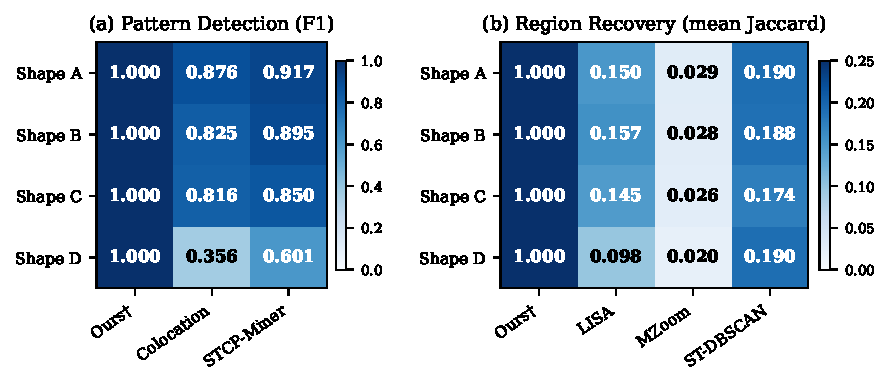
\includegraphics[width=0.90\columnwidth]{fig/fig_ex1_heatmap.pdf}
\caption{EX-1 results (3-seed average, $p_{\mathrm{embed}}{=}0.25$).
  (a)~EX-1-1 F1; (b)~EX-1-2 mean Jaccard.
  GT is the exact solution under the sliding-window definition (Definitions~3--5).
  $\dagger$The proposed method outputs the exact solution by construction,
  hence F1 $= 1.00$ and Jaccard $= 1.00$.
  Baseline parameters were selected by grid search.}
\label{fig:ex1}
\end{figure}

\paragraph{Analysis.}
The proposed method achieves F1\,$=1.00$ and Jaccard\,$=1.00$ by construction,
while existing methods achieve at most F1\,$=0.917$ and Jaccard\,$=0.190$.
---~\textbf{LISA}: collapses occurrences over all time steps, discarding temporal structure.
---~\textbf{MZoom}: Cartesian-product constraint forces convergence to width-1 blocks on a sparse grid.
---~\textbf{ST-DBSCAN}: labels only occurrence cells, missing non-occurrence cells inside dense windows.
These structural mismatches---not parameter tuning---explain
why no baseline approximates the sliding-window definition well across all shapes.

% ==============================================================
\subsection{EX-2: Scalability (Synthetic Data)}
\label{sec:ex2}
% ==============================================================

\paragraph{Objective.}
We evaluate how runtime and peak memory scale
with respect to four parameters independently:
number of temporal grid points $T$,
spatial grid points $S$,
number of dimensions $d$,
and item-set size $|\mathcal{I}|$.

\paragraph{Synthetic data generation.}
On a $d$-dimensional lattice, each item was independently sampled from
Bernoulli$(p_{\mathrm{item}}{=}0.10)$ for all cells to form one basket.
Empty cells were assigned item~1 by default,
ensuring exactly one transaction per cell
(generation details in Appendix~\ref{sec:ex2_data_details}).

\paragraph{Proposed method parameters.}
$W = (24, 4)$ and $\theta = 15$ were fixed throughout.
Base configuration: $T{=}1{,}000$, $S{=}100$, $d{=}2$, $|\mathcal{I}|{=}20$.

\paragraph{Experimental design.}
Four axes are evaluated independently:
(a)~$T \in \{10^2, 10^3, 10^4, 10^5\}$ ($S{=}100$, $d{=}2$);
(b)~$S \in \{10, 10^2, 10^3, 10^4\}$ ($T{=}1{,}000$, $d{=}2$);
(c)~$d \in \{2, 3, 4\}$ with $N{\approx}10^5$ fixed by adjusting spatial dimensions;
(d)~$|\mathcal{I}| \in \{20, 40, 60, 80\}$ ($T{=}1{,}000$, $S{=}100$, $d{=}2$).

\paragraph{Analysis.}
Fig.~\ref{fig:ex2_scalability} shows runtime and peak RSS for all four axes.
Both $T$- and $S$-scalability are approximately linear in $N$:
as $N$ grows from $10^4$ to $10^7$, runtime increases ${\approx}10^3$-fold ($0.046$\,s to $49.5$\,s),
and a higher $T/S$ ratio is slightly faster due to more effective gap-skipping (Lemma~\ref{lem:stride}).
An extended run at $N{=}10^8$ ($T{=}10^6$, $S{=}100$) completes in $517$\,s ($<9$\,min), consistent with linear scaling.
Increasing $d$ from 2 to 4 raises $W_{\mathrm{sp}}$ from 5 to 125 ($25{\times}$),
yet peak memory grows only $1.35\times$, reflecting multiset sparsity per spatial start point.
$|\mathcal{I}|$-scalability is well below exponential,
as Apriori pruning suppresses candidate expansion for non-dense patterns.

\begin{figure}[t]
\centering
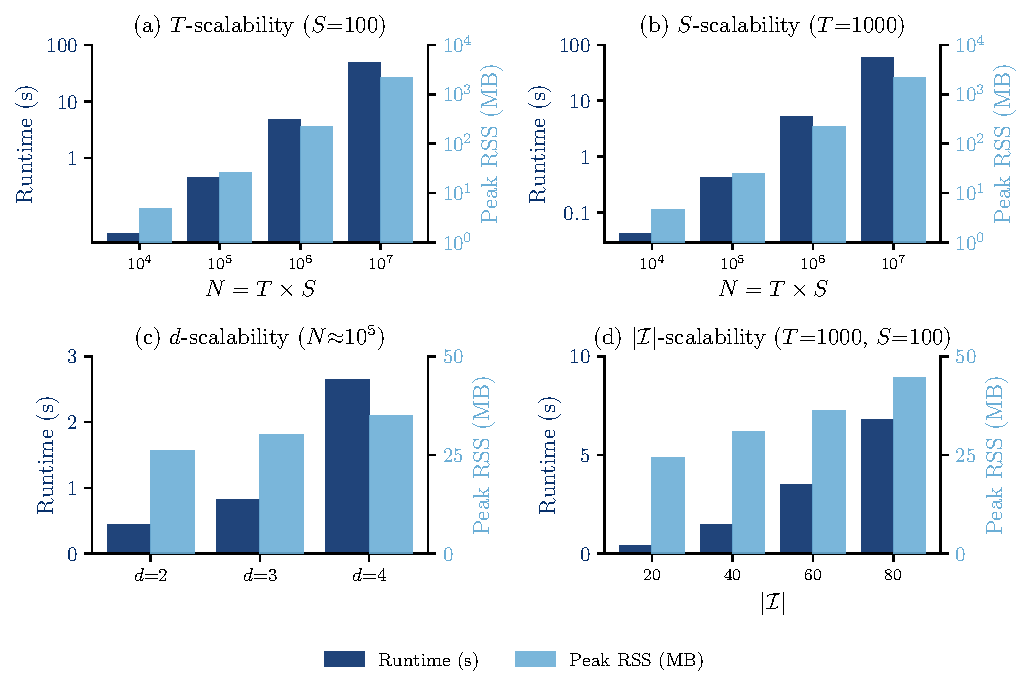
\includegraphics[width=\columnwidth]{fig/fig_ex2_scalability.pdf}
\caption{EX-2: Scalability across four parameters
  ($W{=}(24,4)$, $\theta{=}15$, $p_{\mathrm{item}}{=}0.10$).
  Dark bars: runtime (left axis); light bars: peak RSS memory (right axis).}
\label{fig:ex2_scalability}
\end{figure}

% ==============================================================
\subsection{EX-3: Application to Real-World Data ($d{=}3$--$4$)}
\label{sec:ex3}
% ==============================================================

\paragraph{Objective.}
We applied the proposed method to real-world data from diverse domains
and found that the detected patterns and dense regions
yield interpretable insights consistent with domain knowledge.

\paragraph{Datasets and results.}
Two crime report datasets
(Chicago Crime~\cite{chicagocrime}, NYPD Crime~\cite{nypdcrime}),
citizen complaints (NYC 311~\cite{nyc311}),
and an earthquake catalog (USGS Earthquake~\cite{usgseq})
were used, spanning three domains and $d{=}3$--$4$ dimensions.
Time was discretized into weekly bins and spatial coordinates
into equal-width bins, converting each cell's events into a transaction.
Dataset details and quantitative results
are given in Appendix~\ref{sec:dataset_details}.

\paragraph{Findings.}
Detection counts and runtimes are in Table~\ref{tab:realdata_npatterns} (Appendix~\ref{sec:dataset_details}).
\emph{Chicago Crime} (2,835 patterns):
pairs such as \textsc{Assault}\,+\,\textsc{Battery} form chronic dense windows
in south and west side districts;
three-item patterns (e.g., \textsc{Theft}\,+\,\textsc{Criminal Damage}\,+\,\textsc{Battery})
pinpoint compound hotspots that per-category frequency analysis misses.
\emph{NYPD Crime} (4,478 patterns):
compound co-occurrences of felonies (Felony Assault, Robbery) and
misdemeanors (Petit Larceny, Criminal Mischief)
are captured at borough-and-weekly granularity,
revealing locally concentrated combinations invisible to global frequency rankings.
\emph{NYC~311} (5,130 patterns):
Noise\,--\,Residential and Illegal Parking repeatedly co-concentrate
in residential neighborhoods;
seasonal three-complaint patterns emerge in specific boroughs,
providing week-level actionable signals for policy planning.
\emph{USGS Earthquake} (18 patterns, 4-D):
co-occurrence of M3.0--4.0 and M4.0--5.0 within a depth--time--space window
indicates aftershock sequences;
the depth axis distinguishes shallow crustal events (${\lesssim}30$\,km)
from intermediate-depth intraslab events,
consistent with subduction-zone structure.
In all cases the method outputs \emph{which} itemsets are dense and
\emph{when and where} as concrete windows,
providing interpretable results for domain experts.
